\documentclass[a4paper,english, 11pt]{report}
\usepackage[utf8]{inputenc}
\usepackage[T1]{fontenc}
\usepackage{uiomasterfp}
\usepackage{graphicx}
\usepackage{url}
\usepackage{listings}
\usepackage{xcolor}

\definecolor{codegreen}{rgb}{0,0.6,0}
\definecolor{codegray}{rgb}{0.5,0.5,0.5}
\definecolor{codepurple}{rgb}{0.58,0,0.82}
\definecolor{backcolour}{rgb}{1,1,1}

\lstdefinestyle{mystyle}{
    backgroundcolor=\color{backcolour},   
    commentstyle=\color{codegreen},
    keywordstyle=\color{magenta},
    numberstyle=\tiny\color{codegray},
    stringstyle=\color{codepurple},
    basicstyle=\ttfamily\footnotesize,
    breakatwhitespace=false,         
    breaklines=true,                 
    captionpos=b,                    
    keepspaces=true,                 
    numbers=left,                    
    numbersep=5pt,                  
    showspaces=false,                
    showstringspaces=false,
    showtabs=false,                  
    tabsize=2
}

\lstset{style=mystyle}


\author{Joe Bayer}
\title{TCP PEP}
\subtitle{TCP Performance Enhancing Proxy to Support Non-interactive Applications}
\title{TCP PEP}

\begin{document}

 \uiomasterfp[program={Informatics: Programming and System Architecture}, supervisors={Michael Welzl\and Kristjon Ciko}]
\tableofcontents

\listoffigures

\chapter{Intro}

\chapter{Background}

In this chapter we will present some of the required background knowledge to understand the concepts presented in this paper. Focusing on topics that are outside the common understanding of network programming, especially details of certain congestion controllers and network protocols will be discussed. The rest of the thesis will assume the following topics are known to the reader. 

\section{TCP/IP}
Perhaps the most well known internet transport protocol is the Transmission Control Protocol (TCP). It is known for providing reliable and in-order delivery of packets using acknowledgments and re-transmissions~\cite{Eddy_2022}. It was first introduced in 1974, but is still the most used internet protocol. However, as the demands of the internet have changed, TCP has not. Though TCP has been updated with minor extensions over the years, such as increased initial windows or new options, the core ideas have stayed the same~\cite{rfc8803}.\\

Concepts as the end-to-end argument still play a vital role in how TCP is used in the modern internet. TCP is suffering under the illusion that all logic should be placed on the endpoints as the end to end argument denotes. Even if it spans multiple different domains with varying topologies and demands, especially between wired and wireless domains.
\begin{itemize}
  \item \textbf{Wireless Domain}: A wireless communication domain refers to the transmission of data over a wireless medium without the use of physical connections such as wires or cables between devices. This domain covers a variety of technologies, including 3G, 4G, and 5G for mobile communication, Bluetooth and Wi-Fi for close-range communication, and satellite communication for worldwide communication.
  \item \textbf{Wired Domain}: Unlike a wireless domain, a wired domain provides a steady and reliable bandwidth with low error rates and high throughput. The use of Ethernet and Fiber are typical for wired networks, they enable the transmission of large amount of data over long distances and low signal noise. 
\end{itemize}

\begin{figure}[h] % htbp stand for "here", "top", "bottom", "page"
	\centering
	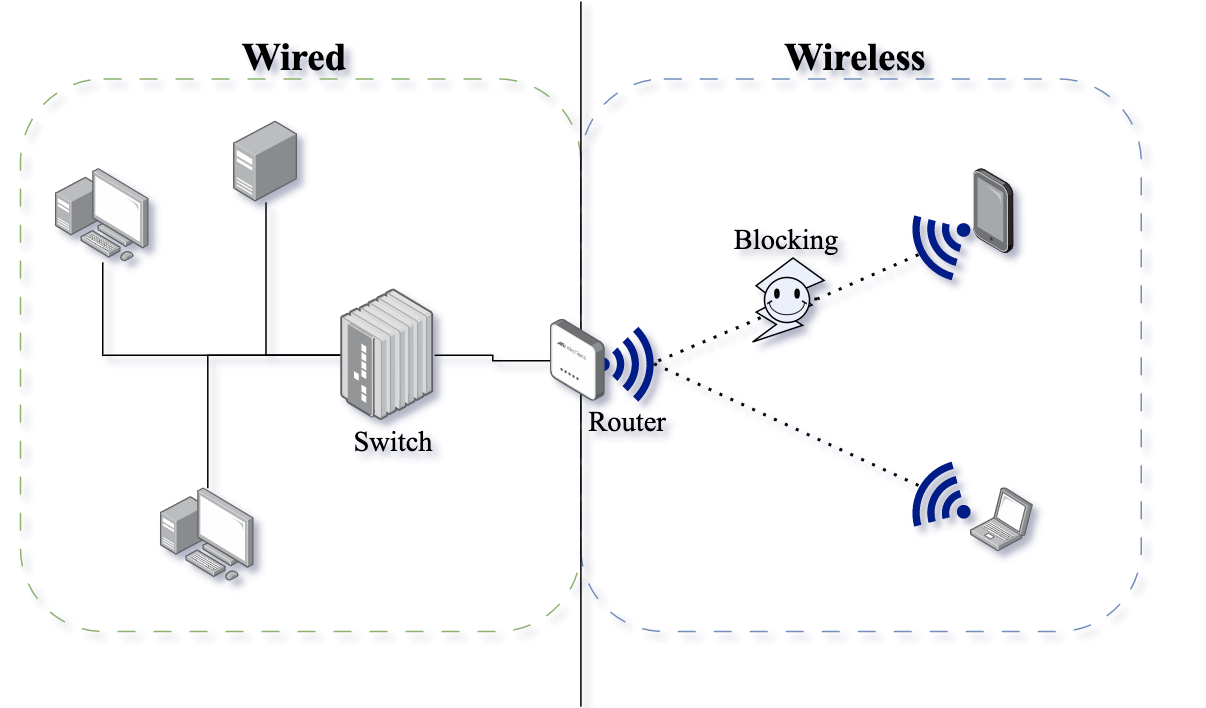
\includegraphics[scale=0.65]{../diagrams/drawio/domains.png}
  	\caption{Example of network domains}
  	\label{fig:domains}
\end{figure}

Each domain has different requirements that a single TCP connection cannot provide. Fig. \ref{fig:domains} shows the two domains and their characteristic differences. Usually, wireless domains experience a lot of changes in connectivity and bandwidths, while the wired domain usually is considered stable. This creates problems for the "modern" TCP which, because of the end to end argument, normally spans multiple domains. Especially congestion control has problems adapting to hight fluctuating bandwidth across long distances and multiple domains.

\subsection{Congestion Control}
Congestion occurs in the internet when a network's resources, such as routers, are overloaded to the point that they diminish quality of the network~\cite{rfc6077}. Packet loss and high delays are common issues associated to high congestion in the network. To solve the problem of congestion, a distributed algorithm is used: Congestion Control. The main goal of congestion control is to maintain a stable network, while still utilizing the available bandwidth shared among all flows. This is achieved by additively increasing the sending rate, and multiplicatively reducing the sending rate when detecting congestion~\cite{welzl_congestion}. Congestion can be detected by packet loss, changes in delay, but also by explicit notifications.\\

Over time different variations of congestion controller have emerged. Although their goal is the same, reduce congestion in the network, their approaches vary. 

\begin{itemize}
  \item \textbf{TCP Reno}: Reno embodies the traditional approach to congestion control. Slowly increasing the sending rate while the network is stable and drastically reducing it on packet loss. TCP Reno was designed for unstable and dynamic networks, where the rapid response rate is crucial to prevent network overloading. However, the slow start rate and aggressive reduction of the sending rate make it sub optimal for more stable networks, where packet loss is less frequent and predictable. Consequently, TCP Reno's reliance on packet loss may lead to unnecessary rate reductions and decreased network throughput.
  \item \textbf{New Vegas}: New Vegas is similar to TCP Reno in most aspects, the main difference is the use of delay to detect congestion instead of packet loss. This makes New Vegas able to react faster to congestion, however it also introduces some interesting side effects. If New Vegas competes with TCP Reno flows, it will start reducing its sender rate before TCP Reno does, this leads to New Vegas losing out on possible bandwidth. 
  \item \textbf{Cubic}: Cubic improves on the idea of TCP Reno by using a cubic function to adjust its (congestion window) sending rate in order to achieve higher throughput in a fast manner. Cubic is very efficient in highspeed networks and known for handling large data transfer over long distances. However, Cubic is not as reliable and robust as more traditional congestion controllers like TCP Reno.
\end{itemize}

In summary, the main differences between TCP Reno, New Vegas and Cubic are their approach to congestion control, their performance in different types of networks, and their trade-off between efficiency and reliability.

\subsection{3 Way handshake (0 RTT)}
For TCP to establish a connection it uses a three-way handshake. Initially, it transmits a synchronization (SYN) packet to the desired endpoint. The endpoint responds with an acknowledgement and a synchronization packet of its own (SYN/ACK). Finally, the client responds with a acknowledgment (ACK). At this point both endpoints have confirmed that they are ready for further communication. For any connection to be established this handshake has to be done. For short flows that terminate in just a few round trips the initial TCP handshake can be a bottleneck, which is made worse if the connection is using a proxy and has to exchange additional information. 

\begin{figure} % htbp stand for "here", "top", "bottom", "page"
	\centering
	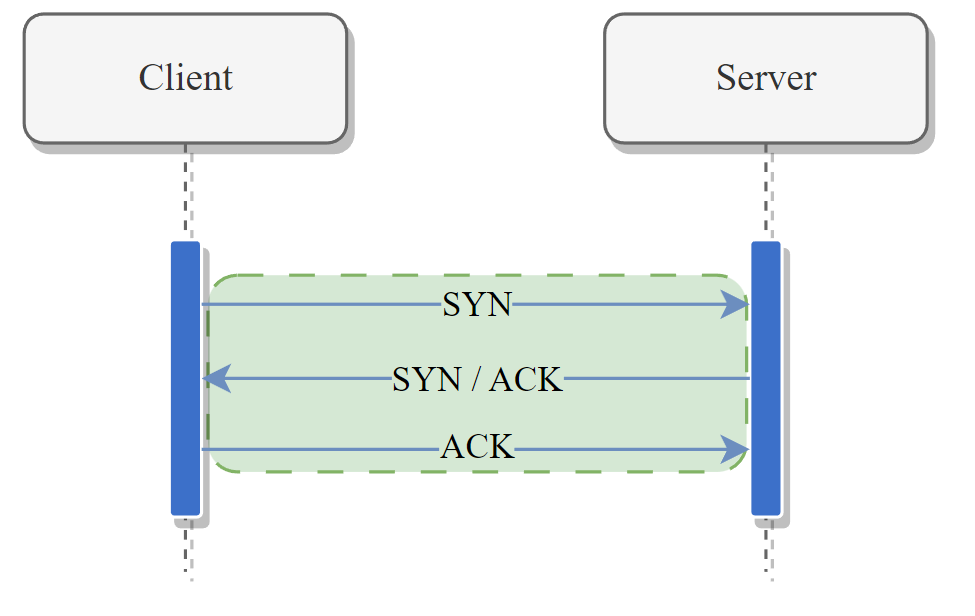
\includegraphics[scale=0.75]{../diagrams/drawio/tcphandshake.png}
  	\caption{The TCP handshake procedure}
  	\label{fig:tcphandshake}
\end{figure}

\subsection{TCP Options and Fast Open}
A TCP connection can be configured with optional header extensions called TCP Options~\cite{tcp_options}. These options change the default behaviour of TCP or add new features. One such feature is TCP Fast Open, which allows data to be added to the initial synchronization packet. A typical use case could be adding a HTTP GET request, thereby saving an entire round trip. In general flows that terminate in a few round trips greatly benefit from this feature. The reason being, the bottleneck in such connections often lies within the initial TCP handshake. Therefore, by removing the extra round trip required to send the first data packet, a significant amount of time can be saved.\\

TCP Fast Open also has other benefits, such as establishing connections to proxies~\cite{rfc8803}. When you are trying to establish a connection through a proxy, you get the added delay of a second round trip sending the desired endpoint. This can be avoided by using TCP Fast Open to send the desired endpoint in the first synchronization packet to the proxy. "SYN forwarding" enables the users to establish a proxy connection without any added delays, however it does depend on the user's application to use TCP Fast Open.

\section{Future of wireless communication.}
The future of wireless communication has seen a lot of improvements such as highly increased bandwidth achieved through advanced technologies like 5G and beyond. Millimetre frequency bands have opened up new possibilities for wireless communication. These higher frequency bands offer greater capacity and can accommodate more devices, however high frequencies come with a set of new challenges such as highly fluctuating bandwidths. This fluctuation can be influenced by various factors such as signal interference, obstacles in the signal path, and environmental conditions.

\subsection{5G Millimetre Wave}
The emergence of 5G Millimeter wave communications has opened the doors for low latency networks with multiple gigabit bandwidth. This is achieved by using higher millimetre wave (mmWave) frequencies in the range of 30GHz to 300GHz, which as a lot of benefits~\cite{Agrawal_Sharma_2016}. A wider spectrum of frequencies to choose from and higher data transfer rates are just some of the many benefits mmWave provides. But along side the benefits, mmWave has also introduced a lot of new challenges.\\

A big problem with millimetre wave communication is signal path blocking also called "Line of sight blocking"~\cite{mmwave_blocking}. It's caused by the use of Beam-forming to increase the bandwidth and range of milimeter wave signals. Beam-forming focuses the signal in a certain direction making any blocking of the signal path devastating for the bandwidth. Even the human body can create enough blockage to drastically reduce the bandwidth. This causes huge fluctuations in the bandwidth whenever the signal is blocked.\\
\begin{figure} % htbp stand for "here", "top", "bottom", "page"
	\centering
	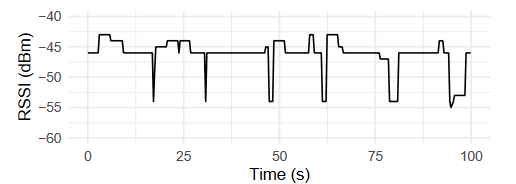
\includegraphics[scale=1.25]{../diagrams/graphs/tcp_mmwave_blockage.png}
  	\caption{5G bandwidth fluctuations from humans}
  	\label{fig:blockage}
\end{figure}

Fluctuating bandwidths lead to unstable TCP connections with a worst case of losing packets. Current TCP congestion controllers such as CUBIC, New Reno or New Vegas struggle when reacting to sudden fluctuating changes. They are simply not able to utilize the high bandwidth when it is available. Simply increasing the aggressiveness of a congestion controller is not an option either as it would disrupt the internet and not be TCP-friendly. A possible solution could be to buffer packets at the 5G base stations, having the data ready for when the bandwidth is high. This however creates a new problem, bufferbloat.


\subsection{Buffering}
\subsubsection{Buffer bloat}
The buffer bloat problem occurs when the systems between the endpoints buffer so many packets that the latency drastically increases and the reliability of the network as a whole goes down. The increased latency is detrimental for interactive (latency sensitive) applications. Generally it's preferred to drop packets and keep buffers small to avoid buffering time sensitive packets such as synchronization packets. Although this works in most cases, it's far from a optimal solution.\\

The increased bandwidth and low latency promises of new technology such as 5G has but a lot of pressure on the efficient forwarding of packets. Small buffers are therefore the standard, But at the same time, fluctuating bandwidth has shown the potential need to buffer packets for non-interactive traffic.
Most focus has been on accommodating for latency sensitive applications like virtual reality or remote surgery to name a few.\\\\
This thesis will explore non-interactive applications where latency is not that critical and more buffering is acceptable and most likely desirable. By splitting traffic into interactive and non-interactive we can improve the performance of both. By having very small buffers for interactive applications we avoid bufferbloat problems, while utilizing the benefits of big buffers for non-interactive applications.\\

\subsubsection{Packet Scheduling}
A method of reducing the effects off bufferbloat is packet scheduling. A system should not send more packets than the weakest link can handle, this idea is built into TCP in the form of congestion control. However, when buffers grow to the point of causing bufferbloat, TCP's congestion control algorithms are unable to confidently determine a sending rate. Packet scheduling can solve this problem as it usually controls the size of the buffers. It makes sure queues can grow when needed, but keep the overall state of the buffers low. Packet scheduling has a lot more to offer than simple queue management, this will be explored later.\\

Proposed packet scheduling algorithms:
\begin{itemize}
  \item \textbf{FQ CoDel}: The Flow Queue Controlled Delay algorithm, FQ CoDel for short, was partly developed to deal with the bufferbloat problem. Its main goal is to reduce the impact of head-of-line blocking and give a fair share of bandwidth by mixing packets from multiple flows~\cite{fq_codel_rfc}. Internally FQ CoDel uses a FIFO queue, classifying packets into different flows to provide a fair share of bandwidth.
  \item \textbf{HTB}: Hierarchical Token Bucket is a queuing discipline based on assgining different classes a certain amount of bandwidth and sending rate. Because of its extensive bandwidth and delay management it's a good option for testing, espeically in a virtual environment.
\end{itemize}

\subsection{Non-Interactive Applications}
Non-Interactive applications such as web traffic, file transfers and video streaming can benefit from larger buffering, especially with fluctuating bandwidths. This is because if we are able to buffer the packets closer to their final destination, we have them ready to be sent when the bandwidth changes. By buffering them we can decrease delay times and acheive faster total completation times for non-interactive traffic.(need citation or prove it myself?). At the same time, interactive applications will not suffer under large queue delays that occur under normal buffering.

\section{Proxy}
Proxy servers play a big role in the modern internet, delivering benefits such as anonymity and increased performance~\cite{nextgen_proxy_servers}. A common use case for a proxy is caching by keeping a copy of popular resources such as a websites. This reduces the latency of accessing the resource as long as the proxy is closer to the user than the original copy. Locality plays an important role in the total latency as any transmission will always be limited by the speed of light.\\

A proxy can also be used for privacy similar to a Virtual Private Network (VPN). By redirecting network traffic through a proxy, the origin of the traffic appears to be the proxy server rather than the actual end-user. Hypertext Transfer Protocol (HTTP), a popular internet protocol used for accessing websites, has this functionality built in using HTTP tunnels and a special CONNECT method in its header.\\

\begin{verbatim}
CONNECT mn.uio.no/:22 HTTP/1.1
Proxy-Authorization: Basic encoded-credentials
\end{verbatim}

\subsection{PEP}
A performance enhancing proxy (PEP) is a connection splitting proxy designed to increase performance of applications using it. The idea behind the PEP is putting more logic such as connection management, buffering, caching inside the network. As the name suggests, a PEP is designed to enhance the performance, but can also introduce new features to a network. An example of a new feature is the multipath support the TCP Transport converter gives.~\cite{rfc8803}.

\subsection{PEP for wireless communication}
Performance enhancing proxies are already deployed and in use for a lot of wireless communication, especially satellites and radio access networks~\cite{tcp_mmwave_proxy}. They have an inherent performance increase just by splitting the connection between the wireless and wired domains. These PEP's are therefore often installed at the base stations. However they are unable to distinguish between interactive or non-interactive traffic, meaning their buffers need to be low and still suffer from fluctuating bandwidth problems.

\begin{figure}[h] % htbp stand for "here", "top", "bottom", "page"
	\centering
	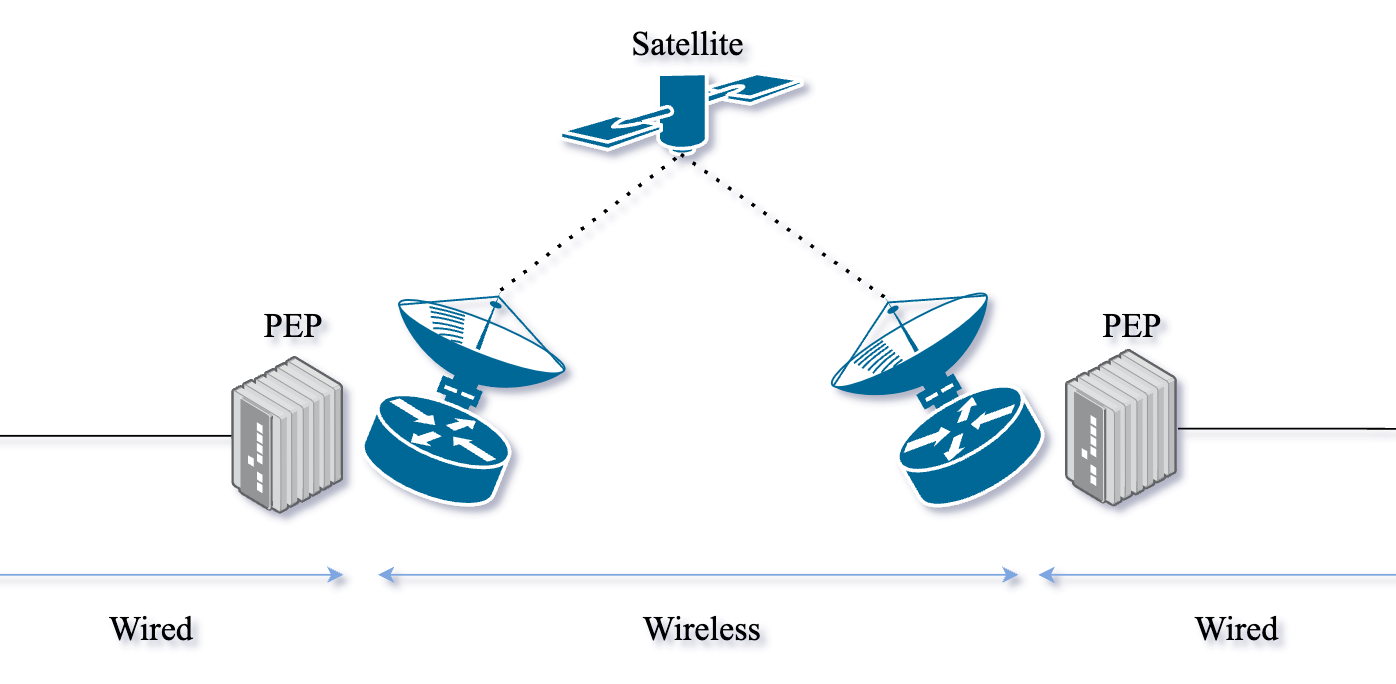
\includegraphics[scale=0.50]{../diagrams/drawio/pep_satellite.png}
  	\caption{PEP installed to support Wireless traffic over satellite.}
  	\label{fig:blockage}
\end{figure}

\subsection{Transparent vs Non-Transparent}
A big discussion regarding PEPs has been if they should be transparent or non-transparent. Transparent PEPs are not visible to the applications that use it. They silently split the connections and spoof the IP-address of both the client and server~\cite{pep_dna}. This is prone to cause unintended side effects, such as certain TCP options not being forwarded and security concerns. Non-Transparent PEPs on the other hand are explicitly chosen by either the client or the server, and the sender is aware of the proxy splitting the original connection. This approach can be seen as more ethical and potentially remove some of the stigma associated with PEPs, this however requires modifications at the sender side utilize the PEP.

\section{Linux}

Linux is the most famous open source kernel freely available for anyone to use and modify. Because of the open source nature of Linux, there have been many various operating system implementation based on the Linux kernel. Ubuntu, Fedora or Manjaro are just some of the most famous Linux based operating systems out there. For developers, Linux is the perfect platform to experiment and test their new innovations. You are able to modify and recompile the kernel itself on the fly, and then test the solution on a live operating system. Linux supports most standards and is used by most major corporations such as Facebook, Amazon, Netflix and Google.

\subsection{Kernel Modules}
Thing that makes Linux truly extensible are Loadable Kernel Modules (LKM). Kernel modules are programs that can be loaded at runtime into the kernel and run with kernel privileges. Running with kernel privileges has a lot of benefits such as having access to internal structures and kernel symbols. Most drivers in the Linux kernel are written as kernel modules as they need access to the system internals.\\

Congestion controllers and packet schedulers are also usually implemented as kernel modules. That is because Linux exposes a struct with function pointers that can be overwritten by a module. Making the kernel call the new functions instead. Because kernel modules run as part of the kernel they do not need to use system call to do basic I/O as using sockets. Removing the overhead of system calls makes the kernel modules run much faster than default user space programs.\\

However, the using Linux kernel modules has the drawback that the program is bound to Linux. The modules will only work in the context of the Linux kernel as they depend on the internal functions, and that they are part of the kernel. Most other operating systems like MacOS will not allow user defined modules to run with kernel privileges. Additionally, any bugs or error in the kernel module with make the entire kernel panic, which usually requires a complete system restart to fix.

\chapter{Design}
A good design for the PEP is crucial as it both needs to be robust, fast and reliable. Not all of the goals are equally achievable, an other aspects need to be considered such as cross platform compatibility. The overarching goal is to improve the completion times of the non-interactive traffic while avoiding to disturb the interactive flows.\\

The second key design aspect focuses on 5G. A goal of the PEP is to better utilize the fluctuating bandwidth, this will influence many aspects such as the placement strategy. This contributes to the overarching goal of making the best use of the new 5G technology.\\

In this chapter we will explore the different ways of achieving our goals and compare them to each other. 

\section{Justification for designing a PEP}

The ossification of networks, particularly TCP, has been a longstanding issue.~\cite{tcp_extendable}\footnote{Cite this} Over the years, the internet has evolved, but the core protocols, like TCP, have remained relatively unchanged. This leads to challenges when attempting to introduce extensions or modifications. Especially, altering such a fundamental protocol could disrupt countless systems and applications. Which leaves us to explore new ideas using middle boxes. A PEP is such a middle box, it can enhance the performance without changing TCP itself.\\

Using a PEP in combination with 5G has additional benefits. Default TCP with 5G needs to cover both the stable network and the fluctuating wireless domain. However, with a PEP we are able to split the domains and perform optimizations, such as congestion control, tailored to each specific domain. Achieving the same optimization by modifying TCP would be a endless close to impossible with the tight integration of end to end congestion control.\\ \footnote{PEPs with 5G, different "domains" works better than normal PEPs}

The development of PEPs have seen a lot of resistance over the years because of the end-to-end argument: keeping logic at the endpoints.\\


\section{PEP Programming}

\subsection{Choosing the Programming Language}
A PEP aims to boost the performance of applications that use it. The speed at which they can process and forward packets is critical. Especially when wanting to utilize the rapidly fluctuating bandwidth of 5G, we need to react as fast as possible. Therefore, the programming language chosen for a PEP has a direct impact on its efficiency. Interpreted languages like Python might not offer the speed necessary for high-performance tasks. Even Java, while running within the JVM, can potentially introduce delays. The languages best suited for high performance are C, C++ and Rust. Both C and C++ are very similar and well suited for high performance systems, Rust has an additional aspect as it supports compile-time checking for race conditions.


\paragraph{The C Programming Language}
C has been the optimal language for high performance systems since its creation in 1972.~\cite{c_programming_language} It was originally created for UNIX when it needed a higher level language, and now is the main programming language behind most operating systems such as Linux, Mac and Windows. Being very close to its predecessor, assembly, and compiled to a binary, makes it one of the fastest languages we have to date. Heap memory management is explicitly done by the programming with no support for garbage collection. The unsafe memory management is one of the main challenges when programming in C, which however can be a benefit because a runtime garbage collection usually results in performance loss.

\subsection{Kernel Module Vs. Userspace Application}
A major design decision is whether to write the PEP as a user-space program or a kernel module. This will also influence the choice of programming languages, because kernel modules mainly are written in C, although Rust has now also been slowly adopted.\footnote{fill inn more} Making system calls (syscalls) can introduce some performance overhead, which is a consideration when looking at user-space programs. In contrast, MacOS offers the kernel extension framework for tasks that require deep system integration, though it comes with its own set of challenges and constraints.\\

Opting for a user-space application has the advantage of being cross-platform, meaning it can run on multiple operating systems without major modifications. On the other hand, a Linux kernel module runs within the kernel space, eliminating the need for syscalls and often offering better performance. However, it's tightly bound to the Linux environment, which might limit its applicability in diverse systems.

\subsection{Optimal Choices for PEP Performance}
Because of the efficiency and possibility of kernel modules, C offers the optimal performance for a PEP. This combination leverages C's high-speed capabilities and the direct kernel integration, minimizing overheads and maximizing efficiency. This choice binds us to the Linux kernel, but this is a small price to pay for salvation.\footnote{Find a actually good way to say this. :) Also! Future work could be comparing to a userspace application? }

\section{PEP Transparency}
Transparent and Non-Transparent PEPs differ in their visibility and interaction with applications. The choice between these two options all have their own set of advantages and challenges. These include ethical concerns regarding transparency, potential issues associated with unaware applications, and considerations for deployment.

\subsection{Transparent}
Transparent PEPs offer an advantage in deployment as they can be introduced without any changes on the client or server end. This ensures that even legacy applications can benefit from the PEP. Also, by nature, the PEP will always be on path of the original connection. However, when unknown middle boxes interfere with a connection, unintended side effects, such as losing TCP Options, become more likely. Furthermore, without knowledge of the PEP, applications cannot modify their behavior, which limits their extensibility.\footnote{Talk more about ethical concerns?}

\subsection{Non-Transparent}
Since applications are fully aware of the PEP when it is non-transparent, we can adjust the PEPs functionality based on the application using it. Applications can also adapt their behavior, optimizing their operations based on the presence of the PEP, leading to potential performance improvements. Although side effect may still occur, applications are aware of them and can actively mitigate them.
Deployment, however, becomes more problematic as for the PEP to be efficient it needs to be on the shortest path which is no longer guaranteed.

\subsection{Choosing a Non-Transparent PEP}
Although transparent PEPs are more common, the goals the TCP PEP aligns more with an non-transparent PEP. The possibilities and potential a non-transparent PEP has is worth breaking the standards.\footnote{This entire sub section should be rewritten, but point stands}
Since the goal is to increase the efficiency of a certain kind of application, non-interactive, it will be important that the PEP can adapt.

\section{Connection Handling in PEP}

\subsection{Connection Splitting}
A performance enhancing proxy does not inherently need to be connection splitting. Depending on its implementation within the network stack, a PEP can buffer and process packets without requiring the termination of the end-to-end connection. A PEP could passively monitor or manipulate the traffic, or or even preemptively transmit ACKs.
\footnote{Picture of a PEP only sending ACKs, perhaps PEP DNA?}\\
\\
There are multiple benefits and disadvantages with using a connection splitting PEP. Firstly, a connection splitting proxy can additionally split the connection into different domains. As discussed in Chapter 2, the internet consist of different domains with their own characteristics. Being able to split the connection into their different domains, enables the PEP to select an appropriate congestion controllers based on the technology and topology of each domain.\\
\\
The connection process to the PEP, and later on the endpoint, is established by informing the PEP of the desired endpoint of the client. This can be achieved by a variety of ways where the goal is to attach additional information to the default connection process of TCP. Preferably, we do not want the overhead of needing an entire additional round trip just to pass this information. Additionally, the client needs to select the PEP, without altering the default socket connection scheme. There are a few different ways of achieving this, which be will discussed below.

\subsection{PEP Selection}
The next challenge is how does a client choose a PEP. We do not want to change the normal socket based scheme of creating a connection, as old applications would need to rewrite a lot of their code. An important prerequisite for the PEP to work is that the PEP is on the shortest path to the chosen endpoint. This can be difficult for an application to be aware of, which leads us to another option. \footnote{How do I solve this? An application does not know the path? So an application cant choose PEP, it can not be system wide as not all connections will have the same path. Although: if its at the access point, all connections will actually go through the it. Discussed in the non-transparent part of design.}

\subsection{Connection Establishment}  
The idea is to attach data to the initial TCP handshake, this way we can inform the PEP of the endpoint without needing to send it with an additional round trip time. Because of the ossified nature of TCP, changing the protocol itself is not an option. The realistic approach is reusing existing TCP functionality to append the desired data. Fortunately, only a small amount of data, less than the usual MTU, is needed to inform the PEP of the endpoint.

\begin{figure} % htbp stand for "here", "top", "bottom", "page"
	\centering
	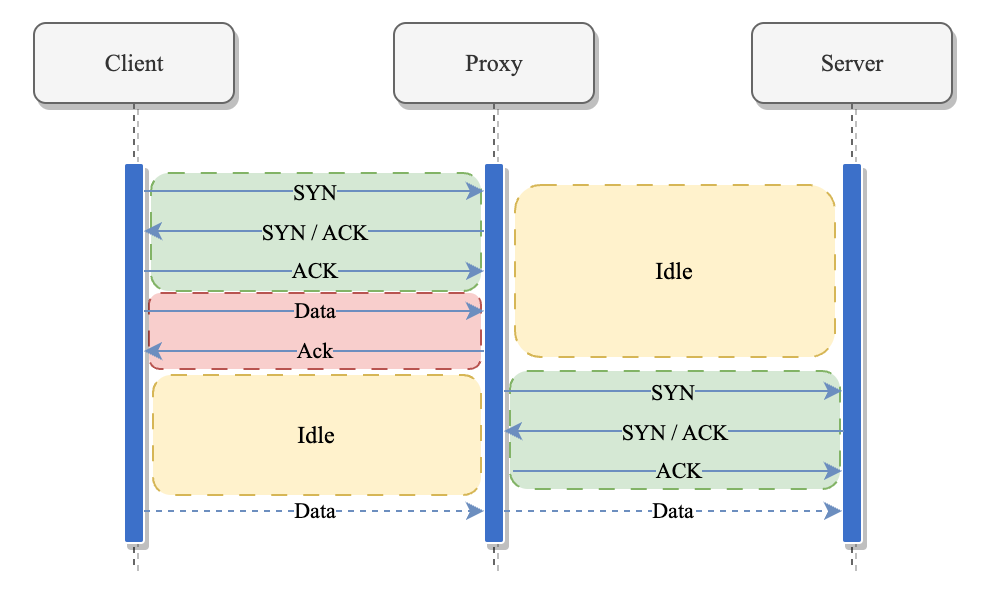
\includegraphics[scale=0.75]{../diagrams/drawio/tcphandshake_primitiv.png}
  	\caption{The TCP handshake procedure across PEP}
  	\label{fig:tcphandshake_primitiv}
\end{figure}

\paragraph{TCP Options}
Since TCP Options can be attached to a TCP connection, a possibility would be to add a new TCP Option which would specify the endpoint. This TCP Option would need to be added by a kernel module, as it is not possible to to add custom TCP Options from user space. This leads to another problem, mainly how to specify from user space that we wish to use the PEP.\\
A possible option would be a socket option, using setsockopt. This however requires changes to the kernel, which raises the bar for adaptability. Another choice would be always attaching the TCP Options on connection addressed to a certain port such as 80/443. This however takes away the choice from the application, and makes it system wide instead.\\

Finally, another significant problem is that unknown TCP Options are often seen as a threat. Firewalls may drop the packets, or the options might be stripped by intermediate nodes.~\cite{middlebox_interactions} This creates a challenge for the implementation and usability of the PEP. If the packets may be dropped because of our custom TCP options, then the PEP will only work in certain networks and scenarios. Although we only design a proof of concept, this is a trade off that is unlikely to pay off in the end.~\cite{tcp_extendable}
\footnote{Directly quote the middlebox interaction paper section 4.4?}

\paragraph{TCP Fast Open}
Another possibility is using the existing TCP Fast Open option which can attach data to the initial TCP handshake. As discussed in the background chapter, using TCP Fast Open can reduce the amount of RTTs needed to establish a connection with both the PEP and endpoint. This requires the socket to be configured and enabled system-wide on the server machine.\\

\paragraph{Optimal Choice}
The most sustainable choice will be TCP Fast Open, adding new TCP Options is simply too unstable. Also, the goal of our PEP is not to change or extend TCP itself. Using TCP Fast Open also has the advantage of being able to add meta data in the size of an MTU, which adds to the adaptability of the PEP to be extended.\footnote{Rephrase last sentence.}

\begin{figure} % htbp stand for "here", "top", "bottom", "page"
	\centering
	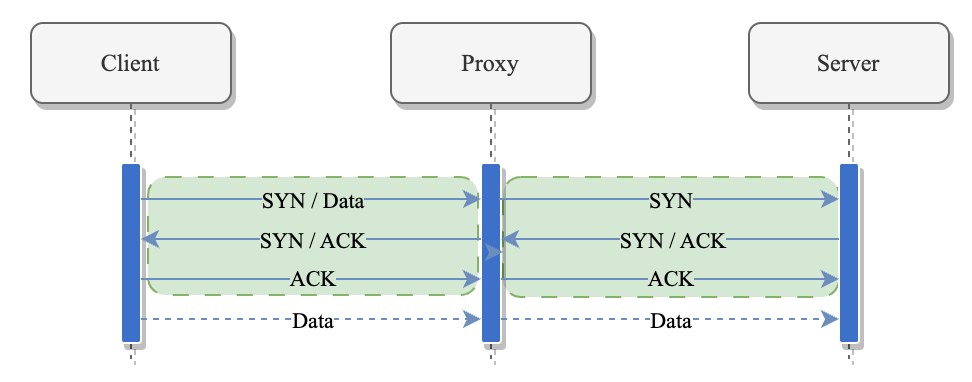
\includegraphics[scale=0.75]{../diagrams/drawio/tcphandshake_optimal.png}
  	\caption{Optimal handshake across PEP (0 RTT)}
  	\label{fig:tcphandshake_optimal}
\end{figure}

\section{Scheduling Algorithms}
The ability to configure and utilize different scheduling algorithms is important for the success of the PEP. This is another choice which will bind us to Linux, as achieving the same control and configuration on other operating system, such as windows or MacOS, will be extremely difficult or even impossible. The impact will be shown in the Evaluation chapter.



\section{Summary}

{Table of design decisions based on different PEP implementations compared to ours.}
{0RTT, Transparent, TLVs, Special ACKS, connection splitting.}\\
\begin{tabular}{ |p{4cm}||p{2cm}|p{2cm}|p{2cm}|p{2cm}| }
 \hline
 \multicolumn{5}{|c|}{PEP List} \\
 \hline
 Implementation& 0RTT &Connection Splitting &Special ACKs &Transparent\\
 \hline
 milliProxy   & AF    &AFG&   004 & x\\
 PEPDNA&   AX  & ALA   &248 & x\\
 SnoopTCP &AL & ALB&  008 & x\\
 Our PEP    &DZ & DZA&  012& x \\
 Transport Converter &   AS  & ASM&016& x\\
 ...& AD  & AND   &020& x\\
 ...& AO  & AGO&024& x\\
 \hline
\end{tabular}

\chapter{Implementation}
This chapter will explore implementation of the TCP PEP, following up on the design choices mentioned in the previous chapter. The development of the PEP will give a deeper understanding of the underlying mechanisms and how they aim to better utilize the 5G bandwidth. All aspects from kernel modules, PEP architectures and additional libraries will be covered.

\section{Kernel Module}
As mentioned in the design chapter, the PEP will be written as a kernel module instead of a normal user-space program. Running and creating a kernel module requires more initial preparation than the a normal application. Firstly, the biggest change is that our PEP will now be a run as a module inside the Linux kernel instead of as a application in its own virtual environment. Injecting a module into the Linux kernel is very different from simply running a binary.\\

A Linux kernel module is loaded and unloaded with the help of two functions that need to be define.

\subsection{Linux Version and Distribution}

\subsection{Implications}

\begin{lstlisting}[caption={kernel\_recvmsg wrapper for receiving for TCP msgs}, label={lst:pep_tcp_receive} ,language=C]
int pep_tcp_receive(struct socket *sock, u8* buffer, u32 size)
{
	struct msghdr msg = {
		.msg_flags = MSG_DONTWAIT,
	};

	struct kvec vec;
	int rc = 0;

	vec.iov_base = buffer;
	vec.iov_len  = size;

	printk(KERN_INFO "[PEP] kernel_recvmsg: calling recvmsg \n");
pep_tcp_receive_read_again:
	rc = kernel_recvmsg(sock, &msg, &vec, 1, vec.iov_len, MSG_DONTWAIT);
	if (rc > 0)
	{
		tlv_print(buffer);
		printk(KERN_INFO "[PEP] kernel_recvmsg: recvmsg returned %d\n", rc);
		return rc;
	}

	if(rc == -EAGAIN || rc == -ERESTARTSYS)
	{
		goto pep_tcp_receive_read_again;
	}

	printk(KERN_INFO "[PEP] kernel_recvmsg: recvmsg returned %d\n", rc);
	return rc;
}
\end{lstlisting}

\section{TLV Library}

\subsection{Shared Libraries}

\section{PEP}

\subsection{Architecture}

\subsection{Kernel Sockets}

\subsection{Client Sockets}

\section{PEP Connect}
Since are PEP is explicitly addressed we need to change how we connect on the client side.
The default approach is to use the \textbf{connect} function, our goal is to imitate this functions behavior, return code and parameters. By keeping our connect function as similar to the original we reduce the overhead of switching over to it. The only change to the original connect that we need is to specify type of traffic, interactive or non-interactive.
\begin{lstlisting}[caption={PEP connection}, label={lst:pep_connect_use} ,language=C]
int socket, ret;
struct sockaddr_in s_in;
bzero((char *)&s_in, sizeof(s_in));
s_in.sin_family = AF_INET;
s_in.sin_addr.s_addr = inet_addr(IP);
s_in.sin_port = htons(PORT);

socket = socket(AF_INET, SOCK_STREAM, IPPROTO_TCP);

ret = connect(server, (struct sockaddr*) &s_in, sizeof(s_in));
ret = pep_connect(server, (struct sockaddr*) &s_in, sizeof(s_in), PEP_INTERACTIVE);
\end{lstlisting}

\section{PEP Connections}

\subsection{Threads Vs. Callbacks}

\section{Memory}



\chapter{Evaluation}

\section{Initial configuration}

Sender --> Receiver --> Receiver
\\
Data being pushed from Sender to receiver, file size, speed, delay.
\subsection{Traffic Control Options}s
Linux has support for network interface configurations using the TC (traffic control) command. TC allows the configuration of packet scheduler, bandwidth, delay and jitter etc. These options combined with the fact that each network interface can have it's own configuration, allows for very precise testing environments. 
\\
fq codel does not allow the configuration of delay, this means we have to configure the delay on the path of the ACKS?
We have to configure the delay on sender facing interface cards. 
\footnote{Picture of testbed setup} 

\subsection{Scheduling Algorithms}
The choice of scheduling algorithm is very important for our test scenarios. As it will greatly affect the results of our tests, we will compare some against each other. The main goal is to highlight the effect and find the optimal algorithms for our PEP.

\paragraph{FIFO}
In our test case FIFO will have the effect of creating up a queue at our PEP. This is detrimental for the interactive UDP flow as it will be stuck in the queue, building up delay. This behavior can be explained by the fact that the non-interactive flow has a much higher sending rate than the interactive flow, thereby quickly filling the finite queue with non-interactive packets.

\paragraph{FQ CoDel: IMPORTANT}
FQ CoDel has a solution for this problem by providing a fair queuing mechanism. 
\paragraph{PFIFO}
Another alternative is Priority FIFO (PFIFO). As the name suggests it combines the concepts of a basic FIFO queue with priorities. This can reduce delay



\subsection{Interactive vs PEP}
Our first experiment consists of having a interactive flow (100 byte UDP packets at 2kBps) competing with a file transfer, one default end to end and one through our PEP. Highlighting some of the initial differences between an end to end connection and a PEP.\\


\begin{figure}[h] % htbp stand for "here", "top", "bottom", "page"
	\centering
	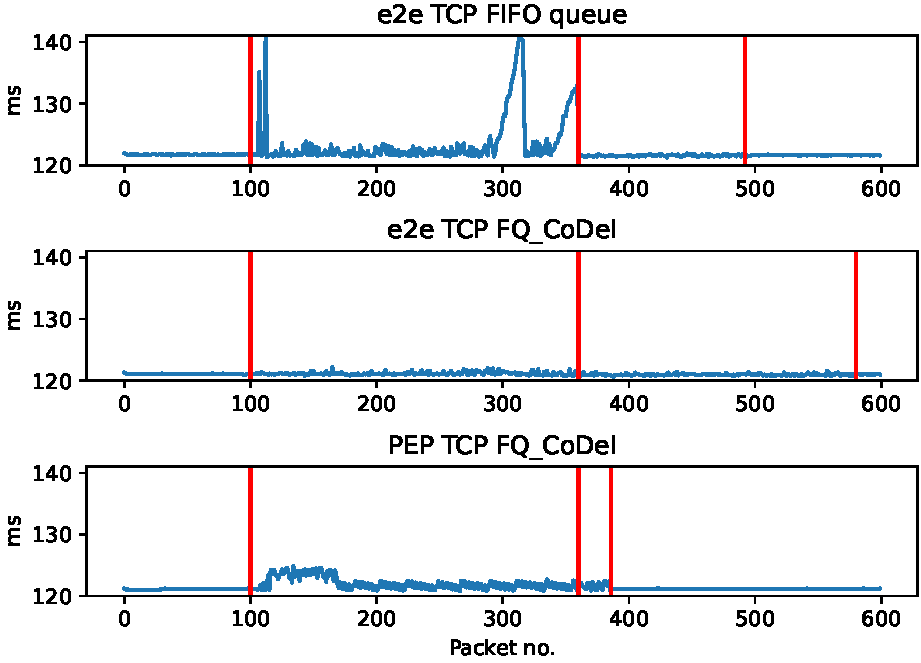
\includegraphics[scale=0.50]{../diagrams/graphs/initial_udp_latency_timeseries.pdf}
  	\caption{Interactive UDP traffic}
  	\label{fig:inital_test}
\end{figure}

\subsection{PEP vs E2E tests}
The first test consists of evaluating our PEP against a default TCP end to end (E2E) connection, while also highlighting the difference a packet scheduler can make. Fig. \ref{fig:inital_test} shows the results, the red lines represent important events in the timeline.
The first line represents the start of a file transfer, the second shows a bandwidth change from 10mbit to 75mbit, while the last line shows when the file transfer finished.\\ 

The first timeline shows an end to end TCP transfer using a FIFO queue, in this case BFIFO.\\ 
On the second timeline we see the behavior of an end to end connection using FQ CoDel. {MORE}
The last timeline shows the PEP using FQ CoDel. Looking at the graph we can see two important differences between the default end to end TCP and the PEP. Firstly, the PEP has higher latency fluctuations than the E2E connection, shown by the blue liens on the graph. 

% FIGURE OF THE TEST SETUP

\subsection{10x10 tests}
To further evaluate the PEP we conducted an experiment where we have 1-10 flows competing, once using the PEP and once end to end. The goal is to see how competing flows affect the behavior of or PEP

\subsection{Spike}

\chapter{Conclusion}

\section{Future Work}

\bibliography{myBib.bib}{}
\bibliographystyle{plain}
\end{document}s
